\chapter{Generative Phonology and its origins}
\label{ch.genphon}

In this chapter, I consider the background and initial progress of
generative phonology from the mid-1950s to about the time {\Chomsky} and
{\Halle}'s \textsl{The Sound Pattern of English} appeared in 1968. There
are two distinct aspects to the issue of how generative phonology
developed during this period, both related to its antecedents. On the
one hand, there is the question of how generative phonology both built
on and replaced other traditions; and, on the other hand, it is worth
examining how generative phonologists dealt with these questions of
origins. This second question is of some interest in the case of this
particular theory, because so much of the early literature of the
field was a conscious attempt to interpret the past—in part to break
with it and in part to renew connections with supposedly forgotten
insights of previous research. The question of the actual (as opposed
to perceived) historical origins of the theory has obvious importance
if we hope to identify those aspects of it that have been taken over
unexamined from other views and maintained well after the basic
assumptions underlying them had been abandoned.

Generative phonology, in particular the work of \name{Noam}{Chomsky} and
\name{Morris}{Halle}, brings together the two principal lines of development
we have been concerned with in earlier chapters. As a student
originally of \name{Zellig}{Harris}, {\Chomsky}'s background was in the most
rigorously formal, procedural, distributional sort of \isi{American
structuralism}. {\Halle}, on the other hand, was a student of Roman
{\Jakobson}, and thus trained in a much different, `European'
tradition. Their collaboration resulted in a theory radically
different from either source, but with essential roots in both.

I will make no attempt in this book to present the principles of the
theory of generative phonology, which may seem strange, given the
historical and theoretical significance of that theory. Other works
exist for this purpose, though, such as
\citealt{goyvaerts.pullum75:essays.on.spe};
\citealt{hyman75:phonology};
\citealt{kenstowicz.kisseberth79:gen.phon};
\citealt{sommerstein77:mod.phon}—most recently,
\citealt{kenstowicz21:spe}---not to mention \citealt{spe} itself, and
the sort of sketch that could be given in a few pages would be of
little use. Instead, my main concern here is to sketch the historical
development of the first years of generative phonology, with
particular reference to the factors that differentiated this new
approach to the field from previous work, and which resulted in the
widespread abandonment of structuralist theory (at least in the United
States) in its favor.

\section{The decline and fall of American structuralism}
\label{sec:decline-fall}
The history of the rise of \isi{generative grammar} (and of generative
phonology in particular) is in large part that of the abandonment of
\isi{American structuralism}. To many non-linguists, the theory of generative
phonology may seem `structuralist' in its essence because it is based
on the premise that structure (and not simply inventory) is paramount
in language; but the particular sense that the term had taken on in
linguistics by the 1950s (both in America and in Europe) was much more
specific, and the replacement of that view by the generative one was a
genuinely fundamental one in numerous ways. The appearance of any new
theory inevitably involves the replacement of older views; but the
relation between American structuralist and generative views was
particularly confrontational. In this section we discuss the early
course of that confrontation, following largely the account given by
\citet{newmeyer:ltia2}.

By the 1950s, linguistics was no longer a marginal field studied as a
part-time interest by scholars whose major responsibility was to some
other discipline. Particularly in the United States, it had become a
thriving subject in its own right, with a substantial number of
faculty and students working in well-established departments of
linguistics specifically on linguistic problems. This new body of
linguists had a strong sense of professional identity, reinforced by
the apparatus of an orthodox academic discipline (a professional
society, annual meetings, the summer Linguistic Institutes, several
journals clearly dedicated to their work, etc.); to a significant
extent, that identity was based on the specific claims of
structuralist theory to a uniquely privileged and scientific view of
an important object of study, human
language.\footnote{\citet{greenberg73:pilot} provides a marvelous
  statement of how successful the US structuralists were (or were
  perceived to be) and why attempts to imitate them in the social
  sciences were failures.} Any new theory questioning basic
structuralist assumptions would naturally have encountered a certain
amount of intellectual resistance, but the resistance in this case was
also to what many saw as a threat to the very foundations of the
field.

To outsiders, American structuralist linguistics in the mid-1950s
seemed to be something of a model science: so well organized, indeed,
that it threatened to find itself out of a job by virtue of having
solved all of its major problems. The basic principles of phonemics
and morphemics had been more or less clarified along lines sketched in
the previous chapter, and the extension of essentially the same
conceptual structure to syntax seemed possible at least in
principle. Given this structure, the main problem for linguistics was
posed as that of developing procedures of analysis applicable to the
data of arbitrary languages, which would yield descriptions of the
desired form. It was generally felt that the bases of these procedures
were already well understood, and that all that remained before
linguistic analysis would be effectively reduced to a mechanical task
(which might even be automated) were refinements in certain relatively
minor details.

Seen from within the field, however, the situation was not quite so
optimistic. From several sides, challenges had arisen which seemed to
undermine important basic assumptions. There was certainly no overall
doubt about the essential correctness of the lines of research being
pursued; but there were nevertheless a number of points on which the
foundations of \isi{structuralism} were potentially vulnerable to a
concerted and coherent attack.

One of these was the set of issues in the philosophy of science which
had furnished such powerful motivation to {\Bloomfield} and the
immediately following generation. In the period between the two world
wars, the operationalist, verificationist assumptions of logical
empiricism had been so dominant as almost to establish the limits of
`scientific inquiry'. Much of the appeal of American structuralist
linguistics was based on its roots in this approach to research, and
the consequent validation of structuralist theory as uniquely
`scientific' in the history of research on language.

By the 1950s, though, philosophers of science were increasingly
questioning the validity of the sort of empiricism to which linguists
had hitched their wagon. It became clear that fundamental scientific
concepts in many fields simply did not have the kind of operational
definition required by the logical empiricists, without thereby being
rendered meaningless. Science in general was becoming more concerned
with the extent to which theories taken as a whole have explanatory
and predictive power within a given domain, bringing coherence and
clarity to it, rather than with the manner in which individual
statements within a theory can be operationally verified. With this
turn, much of the philosophical rationale for the specific conceptual
foundations of \isi{structuralism} crumbled.

In a related development, the approach of radical behaviorists in
psychology was also being questioned. The link between \isi{behaviorism} and
more general issues in the philosophy of science is clear; but it was
specific studies showing the need to posit psychological mechanisms
with more complexity and structure than stimulus-response chains,
rather than the attitude of philosophers, that had begun seriously to
reduce the appeal of \isi{behaviorism} by the
mid-1950s. \posscitet{chomsky59:review_skinner} review of Skinner's
\textsl{Verbal Behavior} was enormously influential in providing a
more or less definitive blow to these views in the specific area of
language, although the process of re-evaluation of their explanatory
power was already well along.

Of course, with the declining acceptance of \isi{behaviorism} came a
willingness to consider more structured and less simplistic
psychological theories in important areas such as perception and
learning. I suggested in chapter~\ref{ch.structuralists} that
acceptance of a particularly limited view of perception seemed to
provide a powerful argument in favor of bi-unique phonemic
\isi{representations}. The notion that (first) language learning takes place
by simple induction against the same assumption-less background as
linguistic fieldwork seemed similarly to validate the procedural
approach to the definition of fundamental linguistic constructs. With
the discrediting of behaviorist assumptions about both perception and
learning, however, came serious weakening of the support for the
theory and methods that American structuralists had appeared to derive
from considerations going beyond linguistics.

Strictly within the field, however, there were also problems to be
noted. An increasing amount of evidence had developed by the mid 1950s
that the strict requirements of a bi-unique phonemic analysis (the
cornerstone of structuralist linguistics) often led to descriptions
that were seriously counter-intuitive.

\citet{bloch41:overlapping} had first addressed this problem in his
paper on ``Phonemic Overlapping'' in which, as discussed in
chapter~\ref{ch.structuralists}, he showed that the requirement of
biuniqueness had the consequence of breaking up the ``neat
parallelism'' of the vowels of \ili{American English} with respect to the
distribution of \isi{vowel length}. In this case, he argued that a proper
understanding of the theoretical construct of the \isi{phoneme} actually led
to an advance: the discovery that the facts were not so parallel after
all. Similarly, in the revision of his analysis of \ili{Japanese} phonemics
between his treatment in \citealt{bloch46:japanese.syntax} and that in
\citealt{bloch50:japanese}, apparently simple and elegant principles
disappear into a welter of particularities. Again, this was hailed as
an advance in understanding that came from the strict application of
biunique phonemic analysis; but structuralist phonemics could really
stand only a certain number of such `advances'. As they accumulated,
it became less and less clear that a theory with such consequences was
actually improving linguists' understanding of the structure of
language.

A particular area in which numerous analytic difficulties arose was
the treatment of \isi{suprasegmentals}: \isi{stress}, \isi{pitch}, and
juncture. Considerable energy, both descriptive and theoretical, was
lavished on these phenomena during the
1950s. \posscitet{trager.smith51:outline} analysis of \ili{English}, with
several distinct \isi{levels} of phonemic \isi{stress} and \isi{pitch} and a set of
junctural elements, was the center of much discussion. As facts in
this domain became clearer (if not clear), two conclusions seemed
ineluctable: first, that the description of supra-segmental phenomena
(at least in \ili{English}, the most extensively studied case) required
extensive reference to grammatical structure if it was to be coherent;
and, second, that the contrasts involved were in no serious sense
recoverable directly from the phonetic data alone.
\citet{lieberman65:intonation} showed experimentally that without
access to other information, even highly trained phoneticians could
not judge \isi{stress} accurately; but this conclusion had long since begun
to force itself on those who worked in the area. The facts of \isi{stress}
(as well as \isi{pitch} and juncture) seemed absolutely intractable within a
theory that required \isi{bi-uniqueness} and that denied the phonology
access to grammatical information.

In fact, the first significant impact of generative work on the
assumptions of American \isi{structuralism} came arguably not from work in
transformational syntax, as is sometimes assumed, but from the
phonological proposals made in \posscitet{chomsky:halle:lukoff} paper
``On Accent and Juncture in \ili{English}.'' They provided an analysis of
\ili{English} \isi{stress} which required only a simple accented/unaccented
distinction in \isi{phonological representations} in place of the four
degrees of \isi{stress} of the {\Trager}-{\Smith} system. The description was
manifestly more elegant than any previous treatment—but it depended
essentially on \isi{rules} that were sensitive to grammatical structure,
applying in cyclic fashion to successively higher \isi{levels} of
constituents in order to derive the complex surface facts from a
simple and straightforward phonemic form.

{\Chomsky}, {\Halle}, and Lukoff\ia{Lukoff, Fred}'s paper established a powerful \emph{prima facie}
case for the necessity of abandoning structuralist assumptions in
order to arrive at a coherent analysis of \ili{English} \isi{suprasegmentals}, but
the defenders of those assumptions hardly rushed to embrace the new
proposals. In 1957, at the Second Texas Conference on Problems of
Linguistic Analysis in \ili{English}, the analysis was vigorously attacked
and (in the opinions of the participants in the conference),
conclusively demolished. Explicit rebuttal of this attack did not come
until {\Chomsky}'s lectures at the {Linguistic Institute} at Indiana in 1964
(subsequently published as \citealt{chomsky66:topics}), but the
issues involved were discussed in various places in the meantime, and
the appeal of the analysis spoke for itself.

In 1958, the organizers of the Third Texas Conference invited {\Chomsky}
to present his work in person, which he did in the form of
\citealt{chomsky62:3texas}. The idea seems to have been to bring all
of the `big guns' of structuralist linguistics to bear on the new
theory, so as to stamp it out before it went too far. The actual
consequences were rather otherwise, however, as a reading of the
transcript of the conference \citep{hill62:3texas} makes fascinatingly
clear. \posscitet[31]{newmeyer:ltia2} description of what transpired
in these sessions as ``{\Chomsky}, the enfant terrible, taking on some of
the giants of the field and making them look like rather confused
students in a beginning linguistics course'' is perhaps something of
an exaggeration, but there is no doubt that {\Chomsky}'s arguments
carried the day, and won him converts. By this time, the emerging
challenge of \isi{generative grammar} to the assumptions of \isi{American
structuralism} had become serious indeed. Even a few structuralists
(such as \name{Robert}{Stockwell}) were coming to be convinced themselves.

\section{The emergence of generative phonology}
\label{sec:emergence}

By the late 1950s, then, the conceptual underpinnings of \isi{American
structuralism} were seriously weakened, and the alternative presented
by a developing theory of \isi{generative grammar} was beginning to make an
impression on the field. The impression should not be given, however,
that structuralist linguistics simply melted away in 1957 or 1958.

\begin{wrapfigure}{r}{.35\textwidth}
  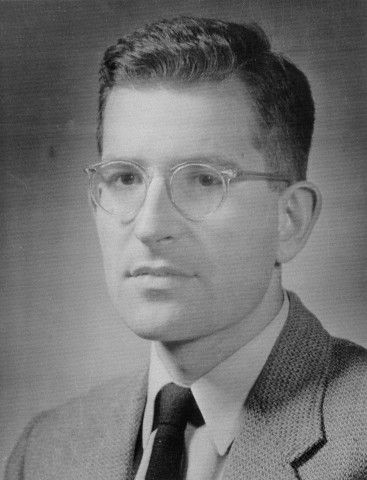
\includegraphics[width=.9\textwidth]{figures/chomsky_1950s.jpg}
  \caption{Noam Chomsky (1950s)}
  \label{fig:ch.genphon.chomsky_1950s}
\end{wrapfigure}
Noam {\Chomsky} was well placed to expose the weaknesses of American
structural linguistics. Born in 1928, his interest in language was
developed as early as the age of ten, when he read the proofs of a
book by his father (the Hebrew philologist \name{William}{Chomsky}) on Hebrew
grammar. At the University of Pennsylvania, {\Chomsky} met \name{Zellig}{Harris}
(whose political views attracted him initially as much as his
scholarship). It was through reading the proofs of
\posscitet{harris:methods} \textsl{Methods in Structural Linguistics}
that {\Chomsky} first learned linguistics. At Penn, he wrote an
undergraduate thesis and subsequently a master's thesis on the
\isi{morphophonemics} of modern Hebrew (\citealt{chomsky51:mmh}; revised as
\citealt{chomsky79:mmh.revised}). This work has the goals of a
\isi{generative grammar}, and deals not simply with \isi{morphophonemics} but with
the entire grammar of the language from syntax through phonology. In
its form a system of ordered \isi{rules} intended to characterize the range
of grammatical sentences in the language, it more nearly resembled the
historical studies of his father than it did the sort of work {\Harris}
was doing. There is little evidence that {\Harris} noticed this, however,
or that he even read {\Chomsky}'s thesis (though {\Chomsky}'s later claims
to this effect are effectively refuted by
\citet[sec. 4.5]{newmeyer22:ailt}). Interestingly, the only linguists
who did show any interest in this work were the Indo-Europeanist 
\name{Henry}{Hoenigswald} at Penn and \name{Bernard}{Bloch} at Yale.

Through the recommendation of the philosopher \name{Nelson}{Goodman}, {\Chomsky}
was appointed a junior fellow at Harvard from 1951 to 1955. This
position gave him essentially complete freedom to work on whatever he
wanted, and at first he pursued the development of the procedural
methods he had learned from {\Harris}. In Cambridge, however, he met
\name{Morris}{Halle} (then a graduate student at Harvard), with whom he spent
a great deal of time in discussion. By 1953, both {\Chomsky} and {\Halle}
had become thoroughly disillusioned with the refinement of
structuralist procedures as a theory of language; and, with {\Halle}'s
encouragement, {\Chomsky} began to work out the ideas underlying his
master's thesis. The result was a manuscript of about a thousand
pages, \textsl{The Logical Structure of Linguistic Theory} (written in
1955-1956, most recently published as \citealt{chomsky85:lslt}) in
which most of the fundamental ideas of \isi{generative grammar} are laid out
and explored.

{\Chomsky}'s recollections that this book was rejected by the only
publisher to whom he sent it are surely not correct: around 1960, he
had two offers to publish it \citep[sec. 4.5]{newmeyer22:ailt},
neither of which came to fruition. He did, however, submit one chapter
of it as a dissertation at the University of Pennsylvania. Thanks to
the influence of {\Halle} and {\Jakobson}, he had a research position at
MIT, where he also taught scientific \ili{French} and \ili{German} and some
undergraduate courses in logic and philosophy. More importantly, he
had the freedom to continue developing his ideas about the foundations
of linguistics in a stimulating and unrestricted atmosphere, with the
collaboration of {\Halle} and others at Harvard and MIT.

\citealt{chomsky57:ss}, a volume based on {\Chomsky}'s notes for an
undergraduate course at MIT \citep[as it is described in]
[63]{chomsky82:generative.enterprise} was published in a new series
which had been started with \posscitet{jakobson.halle56:fundamentals}
\textsl{Fundamentals of Language}. This was \textsl{Syntactic
  Structures}, a work which might have gone essentially unnoticed had
it not been for a review by \name{Robert}{Lees} that was published by {\Bloch} in
\textsl{Language}. \posscitet{lees57:rvw-ss} review forcefully brought
\isi{generative grammar} to the attention of the American linguistic
community, and can be said to have initiated the process of change
that eventually led to the replacement of \isi{structuralism} by generative
grammar in American linguistics.

As a result of his training with {\Harris}, and the amount of attention
he had himself given to the task of defining linguistic structure in
the form of a set of rigorously explicit procedures, {\Chomsky} well
understood the fundamental problems that plagued this approach. On the
other hand, his own education had been thoroughly independent, and his
first substantial results (in \textsl{The Morphophonemics of Modern
  Hebrew}) were achieved without substantial reference to
structuralist assumptions. When he became disillusioned with {\Harris}'s
program and convinced that the effort was necessary, he was thus in a
better position to strike out in a radically different direction than
were those with a more personal commitment to \isi{structuralism}.

One of the strongest points of \isi{American structuralism} was its concern
for formal analysis and explicit statement. Thanks in large part to
{\Chomsky}, this continued to play a central role in \isi{generative grammar},
even though most of the substance of the structuralist position was
replaced. However, given his talent for devastatingly rigorous
argument and analysis, the effect when he did attack the established
view was dramatic.

{\Chomsky}'s proposals quickly became the center of syntactic discussion,
after the appearance of \textsl{Syntactic Structures} and {\Lees}'s
review of this book. To a considerable extent, however, the impact of
\textsl{Syntactic Structures} can be attributed to the fact that
structuralist linguistics simply didn't have a serious `theory' of
syntax. There was general optimism that one was possible as `an
extension of morphology by other means' (to paraphrase von
Clausewitz\ia{von Clausewitz, Carl Philipp Gottfried}), but 
little of substance can really be said to have been
accomplished. Some linguists (such as {\Hockett}, who later became an
outspoken critic of \isi{generative grammar}) were quite ready to see
transformational syntax, in fact, as an approach that could be
directly incorporated into structuralist descriptions in the form of a
new analytic technique requiring only minimal modifications in the
basic assumptions of the theory.

The situation was completely different in phonology, however. Here
there was no sort of theoretical vacuum to be filled: this was
territory that \isi{structuralism} was generally felt to have conquered for
scientific study, and where it was felt to be
strongest. \posscitet{chomsky:halle:lukoff} paper had seriously
questioned the tenability of the basic proposition that phonological
structure was independent of grammar, but the Texas conferences of the
following two years showed that the established figures in the field
were largely unwilling to accept this result—even in the absence of a
genuine alternative in the description of \ili{English} \isi{stress}. At the 1959
Fourth Texas conference, {\Chomsky} was again invited, and this time
presented a paper \citep{chomsky59:4texas} which included discussion
of \ili{English} phonology extending the arguments of
\citealt{chomsky:halle:lukoff}; it is significant (and perhaps no
accident, though the facts are unclear) that the proceedings of this
conference were never published.

At roughly the same time, \posscitet{halle:spr} \textsl{Sound Pattern
  of Russian} extended the attack to the bases of the \isi{bi-uniqueness}
condition, but again acceptance of this critique by the main stream of
American linguistics was anything but
immediate. \posscitet{ferguson62:rvw.spr} extensive and detailed
review, for example, praised the book for providing a clear account of
the emerging theory of generative phonology and of the \isi{acoustics} of
\ili{Russian}, but goes on to attack most of the premises of that theory,
adding that the book ``makes no significant new contribution to our
understanding of the \ili{Russian} sound system'' (p. 284).

In 1962, the {International Congress of Linguists} was held in
Cambridge, Massachusetts. \name{Zellig}{Harris} had been asked to give one of
five plenary session papers but turned down the invitation; the
organizers of the Congress (including \name{Morris}{Halle}) then asked {\Chomsky}
instead. {\Chomsky} devoted a large portion of his paper ``The Logical
Basis of Linguistic Theory'' (subsequently published in various
versions, eventually as \citealt{chomsky64:cilt}) to an extended
criticism of the assumptions of structuralist (or `taxonomic')
phonemics. The aggressive tone and forceful argumentation of this
paper were set in a context which made it clear that the problems it
raised were by no means matters of mechanics, to be solved by a
further refinement of structuralist procedures, but rested on the same
basic issues that were being challenged by transformational theories
in syntax. Such a linking of the two was essential if the
philosophical impact of \isi{generative grammar} was not to be trivialized
by being restricted to those parts of language that structuralists
just hadn't gotten around to yet. Those who would attempt to treat
transformational syntax as a technique to be grafted onto a
structuralist phonology and morphology were forced to face the fact
that those areas were equally challenged—which many were unwilling to
do.

Two other short papers by \citet{halle62:pigg,halle64:bases}, devoted
to the role of \isi{distinctive features} in phonological analysis and other
foundational questions dividing structural and generative phonology,
further presented the case for a generative approach to
phonology. {\Halle} argued that \isi{phonological rules} were more economically
formulated in terms of features than of unitary phonemes; that the
order of application of \isi{rules} provided more insightful formulations,
and indeed that dialect differences could be characterized in terms of
differential ordering of the same \isi{rules}, and other such
points. However, while many younger scholars had become convinced of
the importance of the theory by this time, the field (and its
institutions, such as the annual meetings of the LSA) continued to be
dominated by structuralist studies. Nonetheless, generative
grammarians were increasingly on the attack, at meetings and in
articles and reviews in the principal journals.

The climax of this confrontation can probably be marked as 1965. In
that year, \name{Fred}{Householder} published a long, strongly worded attack
on generative pho\-nology \citep{householder:recent_claims} in the first
number of the new \textsl{Journal of Linguistics}, an article which
summarized virtually all of the objections and grievances against the
new theory that were current in the field. The editor of the journal,
\name{John}{Lyons}, asked {\Chomsky} and {\Halle} in advance of the appearance of
{\Householder}'s paper whether they would like to reply. {\Chomsky} and
{\Halle} were then at work on \textsl{The Sound Pattern of English}, and
Lyons\ia{Lyons, John}' invitation presented them with an opportunity to deal with the
polemic issues surrounding generative phonology in isolation from the
positive statement that the book would make. They therefore agreed,
and the resulting reply \citep{chomsky:halle65:householder_reply},
which appeared in the immediately following issue, provided a detailed
and—for most—conclusive response to the structuralist criticisms.

After 1965 there were still attacks from the structuralist side
\citep[e.g.][]{hockett68:state.of.the.art,lamb66:stratificational.grammar},
but with the exception of a vigorous counterattack by
\citet{postal68:aspects}, a manuscript which had been circulating in
pre-publication versions for at least three years before, generative
phonologists simply failed to pursue the controversy after that. As far
as the determination of the major direction of subsequent research was
concerned, the issue was settled. {\Chomsky}'s effective lectures on
 phonology and syntax (on alternating days) formed the primary focus of
the 1966 {Linguistic Institute} at UCLA, an event organized by the
one-time structuralist turned ardent generativist \name{Robert}{Stockwell},
and consolidated the central position of \isi{generative grammar} (including
phonology) in American linguistics. A number of new departments were
created more or less \emph{ex nihilo} during the 1960s, largely as a
result of the tremendously increased interest in the field which the
new theory of \isi{generative grammar} brought about. A certain number of
more traditional linguistics departments in the United States
maintained a core of (often vocal) structuralist opponents of the new
trend, but these figures found themselves increasingly isolated and
unattended to by the great majority, especially those in the newly
created (and thriving) departments.

\section{Morris Halle and the bases of generative   phonology}

\name{Morris}{Halle}, was born as Moris Pinkovics in Liepāja, Latvia on 23
July, 1923, and had a rather different background from
{\Chomsky}'s.\footnote{Much of the content of this section is adapted
  from \citealt{sra00:royaumont} with permission.}  After emigrating
to the United States with his family from Riga in 1940, he studied
engineering in New York until he was drafted in 1943. After the war,
he attended the University of Chicago, where he received a degree in
linguistics; in 1948, he went to Columbia to study with {\Jakobson}, and
came with {\Jakobson} to Harvard the next year. He was thus a part of the
circle of talented young Slavicists around {\Jakobson} during these
years, and collaborated with {\Jakobson} on a number of influential
works. His Harvard Ph.D. thesis in 1955 was entitled ``The \ili{Russian}
Consonants: A Phonemic and Acoustical Study.''

\begin{wrapfigure}[13]{l}{.35\textwidth}
  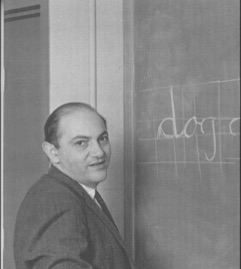
\includegraphics[width=.9\textwidth]{figures/halle_1960s.jpg}
  \caption{Morris Halle (1950s)}
  \label{fig:ch.genphon.halle_1960s}
\end{wrapfigure}
On the basis in part of his engineering background, {\Halle} held an
appointment in the Research Laboratory of Electronics at MIT while he
was a student at Harvard. He was subsequently (in 1951) hired by the
MIT department of modern languages to teach \ili{German} and \ili{Russian}.  A
part of his research on \isi{acoustics} at MIT while he was still a student
involved collaboration with {\Jakobson} and \name{Gunnar}{Fant}, and resulted in
\textsl{Preliminaries to Speech Analysis}
\citep{jakobson.fant.halle52:preliminaries}, a formulation of the
Jakobsonian distinctive-feature framework in simultaneous acoustic and
articulatory terms. {\Halle}'s initial reputation was earned as an
acoustic phonetician, and only secondarily (through his association
with {\Jakobson}) as a phonologist.

\begin{wrapfigure}[11]{r}{.45\textwidth}
  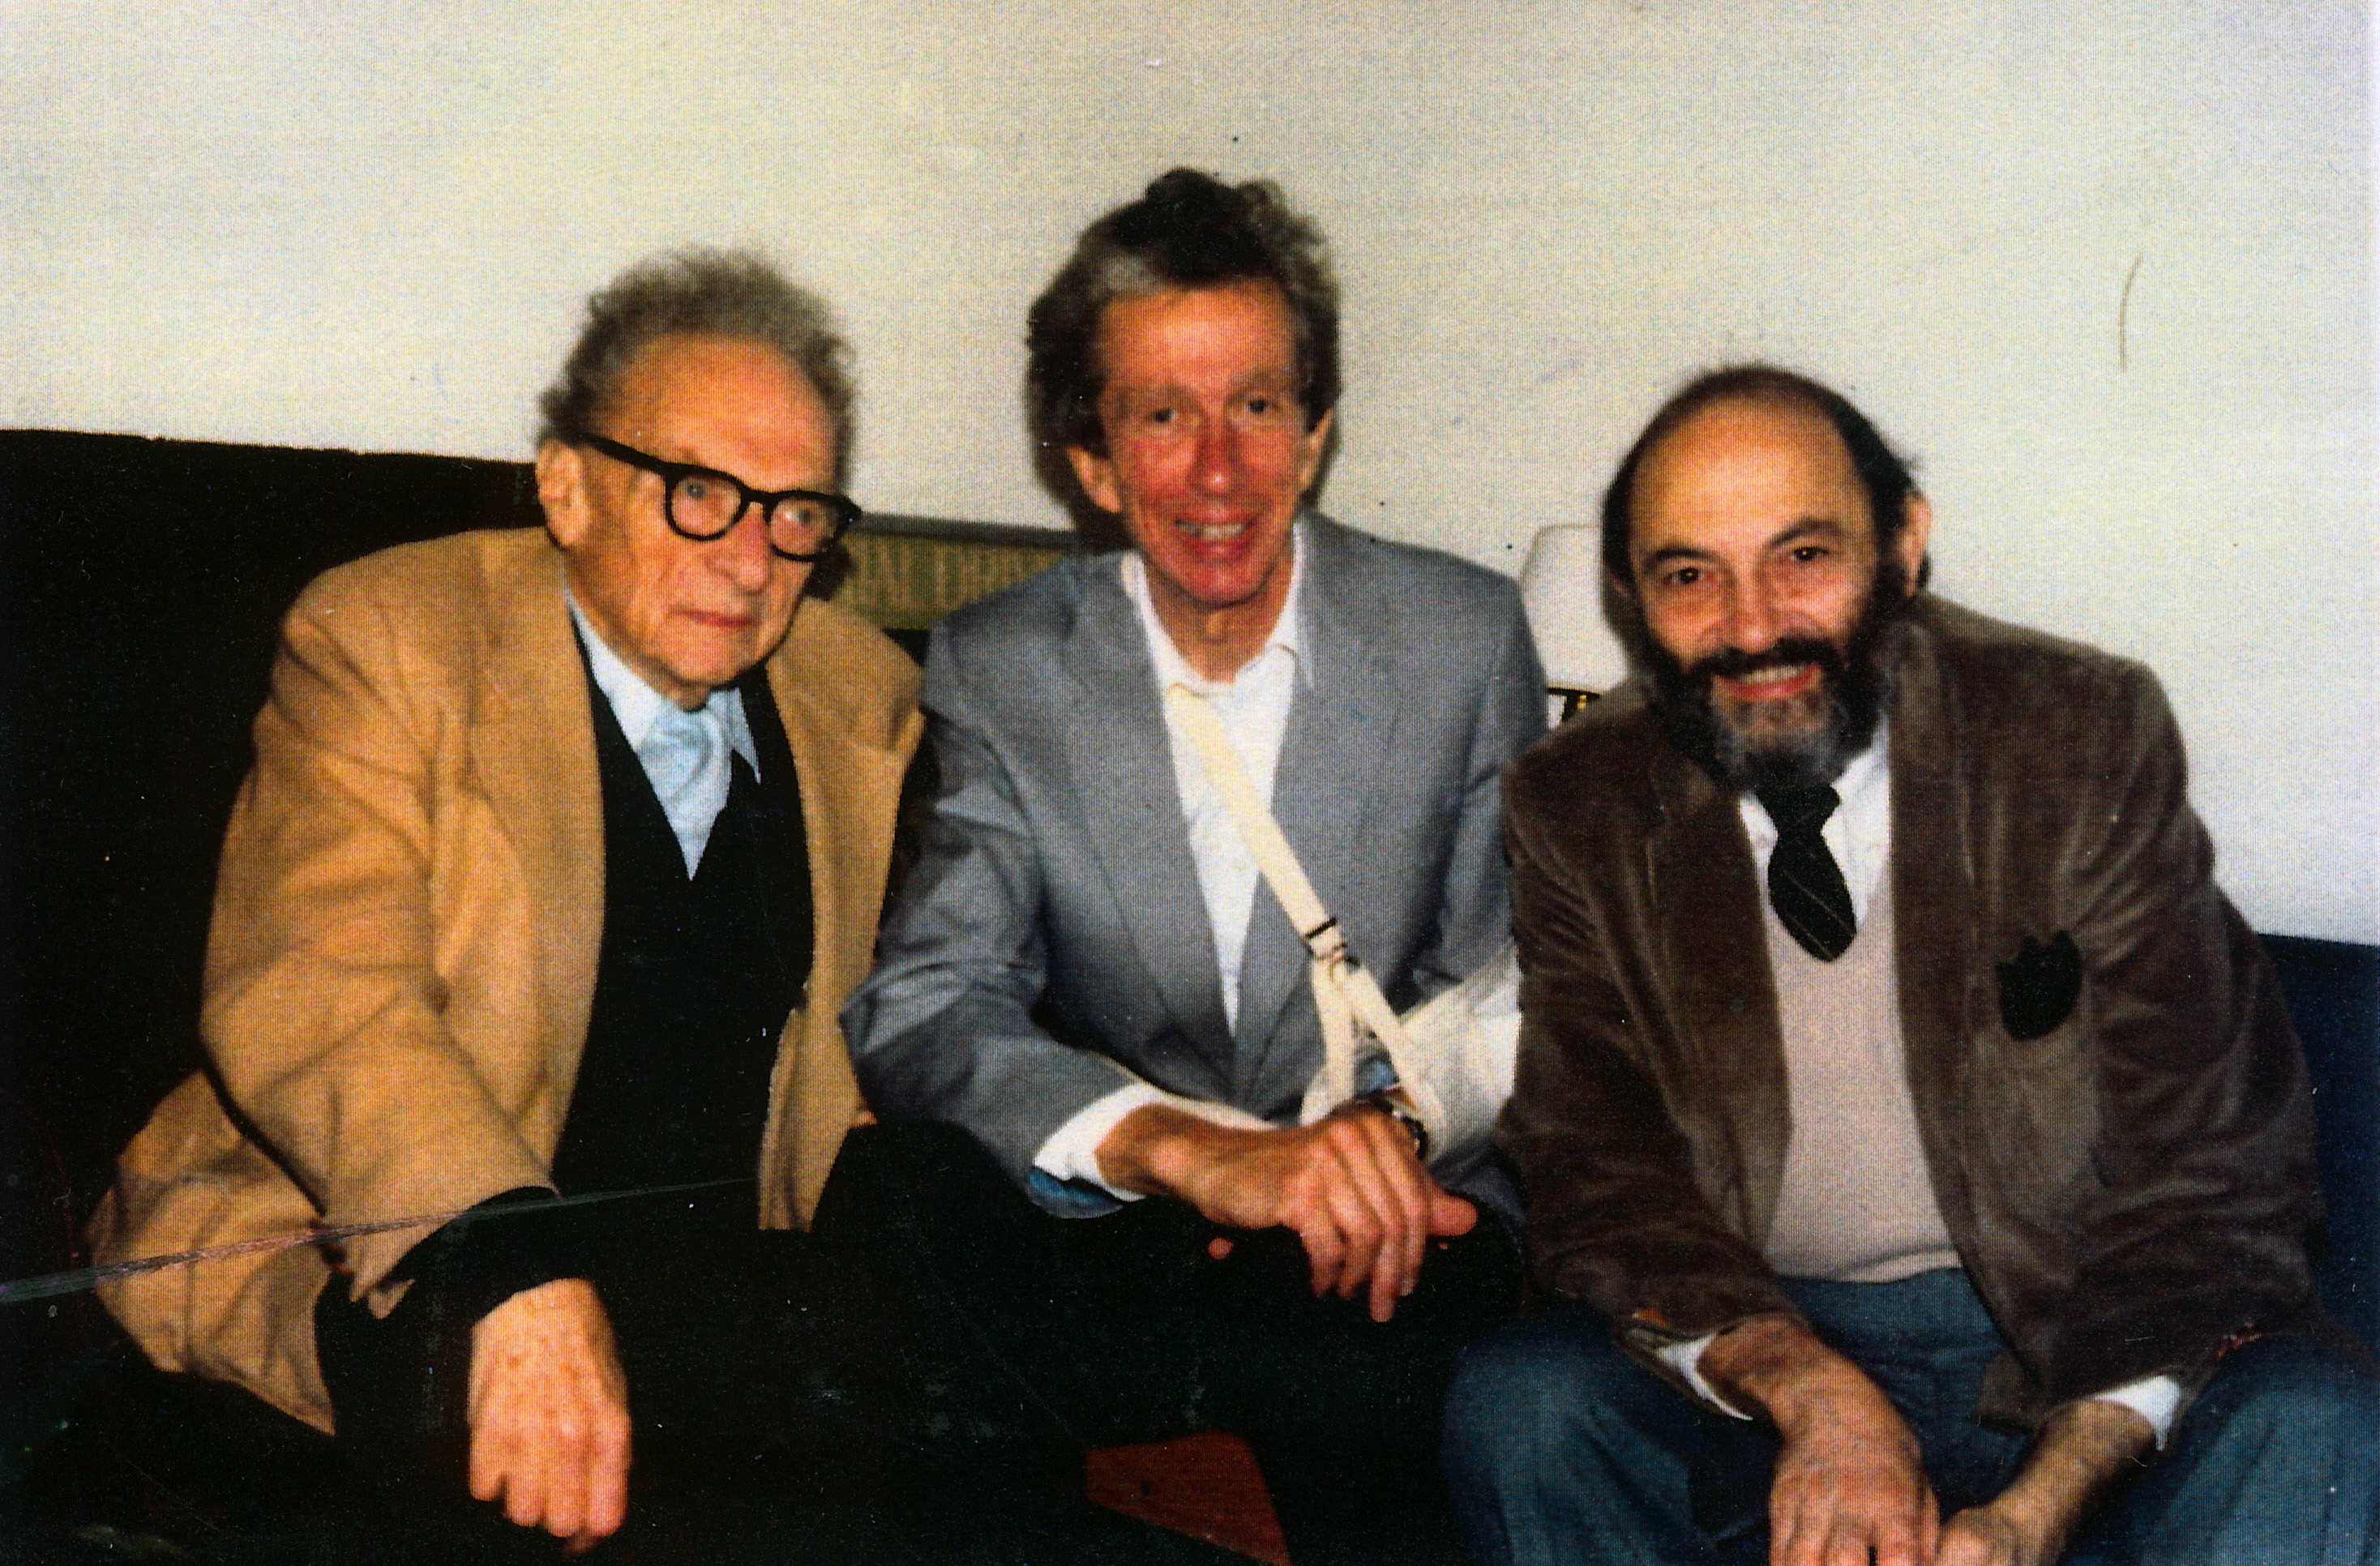
\includegraphics[width=.9\textwidth]{figures/Jakobson_Fant_Halle.jpg}
  \caption{Jakobson, Fant and Halle (ca. 1970)}
  \label{fig:ch.genphon.jakobson_fant_halle}
\end{wrapfigure}
Although {\Jakobson} was particularly interested during the early 1950s
in providing an explicit acoustic basis for the \isi{distinctive features},
he had also done some particularly elegant work on the \isi{morphophonemics}
of Slavic languages (particularly his article ``\ili{Russian} Conjugation,''
\citealt{jakobson48:russian.conjugation})— work which was virtually
ignored by American linguists other than Slavicists at the time. {\Halle}
was greatly impressed and attracted by this work, but also struck by
the difficulty of relating anything like an adequate morphophonemic
representation of utterances directly to the acoustic facts. The
morphophonemic analysis had such obvious coherence and explanatory
value that it seemed inconceivable to deny its importance in the
structure of language, as most American phonemicists attempted to do;
but on the other hand, if this analysis did indeed have a real role in
linguistic structure, its relation to the physical signal must be much
less direct than was posited for a structuralist phonemic
representation.

The several aspects of this problem are addressed in \textsl{The Sound
  Pattern of Russian} \citep{halle:spr}. Indeed, the many distinct
areas which this book deals with in combination make it rather strange
reading today: we are unused to finding a combination of general
linguistic theory and detailed analysis of the phonology of a specific
language together in a single volume with an introduction to the
physical \isi{acoustics} of speech and detailed acoustic description of the
surface segments of the language. All of these are central to {\Halle}'s
project, however. He had decided that morphophonemic representation
was extremely important to the structure of language; but (reflecting
another influence from {\Jakobson}) he believed that a representation
which was perceptually recoverable from acoustic data was important as
well. His goal was to show how these two \isi{levels} of description were
related to each other, and what characteristics each level had. Since
linguists were not generally acquainted with the results of the
rapidly developing theory of the \isi{acoustics} of speech, it was necessary
to give an introductory sketch of this area in order to make his
results comprehensible.

Though it is not, perhaps, the most readable part of this book, the
section for which it is primarily remembered is the introduction to
the first chapter, ``A Theory of Phonology.'' Here {\Halle} lays out a
number of assumptions claimed to be necessary to an adequate
phonological theory; but, most importantly, he argues that a level of
representation meeting the specific conditions of structuralist
phonemics (in particular, the \isi{bi-uniqueness} condition) cannot
naturally be incorporated into such a theory.

In order to account for ``ambiguities due to homophony''
\citep[23]{halle:spr}, a morphophonemic representation is
indispensable; and a universal phonetic representation is similarly
necessary to express the facts of speech. The latter is, for {\Halle},
one in which all of the features in a universal inventory—for example,
the Jakobsonian system—are specified in a way that has a direct
acoustic and articulatory interpretation. In {contrast} to both of
these, a structuralist phonemic representation has the property of
specifying all and only the distinctive sound properties of an
utterance, while still being recoverable from phonetic data alone
(i.e., it meets the condition of \isi{bi-uniqueness}). {\Halle}'s argument was
that such a representation can not in general be incorporated in an
analysis without resulting in ``an unwarranted complication which has
no place in a scientific description of language''
\citep[24]{halle:spr}.

This argument is the basis of a sort of creation myth that grew up
with about the history of phonology, which has structuralists in
America (and also in Europe) concentrating on the discovery of
phonemes as minimal units of surface \isi{contrast} through the 1930's,
1940's and 1950's. Then at the end of the 1950's, {\Halle} presented data
from \ili{Russian} (concerning \isi{voicing} \isi{assimilation}) from which it was clear
that such a notion of phonemes was indefensible and led inevitably to
loss of generality. As a result (with allowances for entrenched
prejudices and the time necessary to re-tool), phonologists
re-oriented their attention toward the previously marginalized domain
of \isi{morphophonemics}, and phonemics was replaced by generative
phonology.

To what extent does that picture correspond to reality? Let us look at
the facts, historical and linguistic. {\Halle}'s argument was first
presented at the 1957 LSA meeting \citep{halle:1957lsa}. Thanks to
the fact that in that era, meetings of the Linguistic Society were
sufficiently small that minutes could be kept showing who attended,
who participated in discussion, etc., we know that in the session at
which this paper was given, about 160 people, including many of the
major names in American Structuralist linguistics of the period, were
present in the audience. The original text is no longer available, but
the form of the argument was apparently the same as that which first
appears in print two years later in \textsl{The Sound Pattern of
  Russian}:
\begin{quotation}
  In \ili{Russian}, \isi{voicing} is distinctive for all obstruents except /c/,
  /č/, and /x/, which do not possess voiced cognates. These three
  obstruents are voiceless unless followed by a voiced obstruent, in
  which case they are voiced. At the end of a word, however, this is
  true of all \ili{Russian} obstruents: they are voiceless, unless the
  following word begins with a voiced obstruent, in which case they
  are voiced. E.g., {[m'ok l,i]} `was (he) getting wet?', but {[m'og
    bɨ]} `were (he) getting wet'; {[žeč l,i]} `should
  one burn?', but {[žeǯ bɨ]} `were one to
  burn'.
    
  In a phonological representation that satisfies both condition (3)
  {[pho\-ne\-mic$\rightarrow$phonetic determinacy---SRA]} and (3a)
  {[phonetic$\rightarrow$phonemic de\-ter\-minacy---SRA]}, the quoted
  utterances would be symbolized as follows:\\/m'ok l,i/, /m'og bi/,
  /žeč l,i/, /žeč bi/. Moreover, a rule would be required stating that
  obstruents lacking voiced cognates --- i.e., /c/, /č/, and /x/ ---
  are voiced in position before voiced obstruents. Since this,
  however, is true of all obstruents, the net effect of the attempt to
  meet both condition (3) and (3a) would be a splitting up of the
  obstruents into two classes and the addition of a special rule. If
  condition (3a) is dropped, the four utterances would be symbolized
  as follows: \{m'ok l,i\}, \{m'ok bi\}, \{žeč l,i\}, \{žeč bi\}, and
  the above rule could be generalized to cover all obstruents, instead
  of only \{č\}, \{c\} and \{x\}. It is evident that condition (3a)
  involves a
  \isi{significant} increase in the complexity of the representation.\\
  \citep[22f]{halle:spr}
\end{quotation}
  
{\Halle}'s argument is standardly adduced as having persuaded
phonologists to abandon the phonemics of the time, and take up the
rather different pursuits of generative phonology. The logic of the
argument is that a description interposing a level of representation
meeting the `\isi{bi-uniqueness}' condition between the morphophonemic and
\isi{phonetic representations} leads necessarily to a situation in which a
regularity of the language, the \isi{assimilation} of \isi{voicing} in clusters of
obstruents, cannot be stated in a unitary way. As I will argue below,
the force of this argument rests in its focus on the need for a
grammar not only to assign the correct \isi{representations} to linguistic
forms but also to give an account of the \emph{rules} of the language,
\isi{rules} which correspond directly to components of a speaker's
linguistic knowledge. The extent to which that logic was actually
apparent to the linguists of the time who heard it is not obvious
however, as we will see.  My concern is to understand just what the
relation was between this argument and the subsequent change in the
subject matter of phonology.
  
It is reasonably clear that the role of {\Halle}'s argument cannot have
come from the novelty of the facts whose analysis was at issue, since
similar material had been discussed before, as noted by
\citet[288]{ferguson62:rvw.spr}. {\Halle}, indeed, cites one such
instance (though curiously, not one of the better known cases I will
cite below: the fact that {\Halle} mentions only Matthews\ia{Matthews, G. H.} in this
connection, and not {\Bloch}, {\Bloomfield}, or some other structuralist has
been adduced by some as presaging a narrowness in citation practice of
which generative linguists are still accused):
  
``Analogous examples can be cited from many languages. An especially
interesting example is discussed by G. H. Matthews, ``A Phonemic
Analysis of a \ili{Dakota} Dialect'' {[\citealt{matthews:dakota_phonemics}]}, who
shows that the labial and dental \isi{nasal consonants} are automatic
alternants of the cognate \isi{stops} as well as of /m/ and /n/, while the
velar nasal is an alternant of the velar stop exclusively.''
{[\citealt[22, fn. 12]{halle:spr}]}
  
In fact, the example {\Halle} refers to is \emph{not} analogous in the
relevant details to the \ili{Russian} case. Matthews shows that /b, t, k/
are replaced by {[m, n, ŋ]} in syllable-final position after a
\isi{nasal vowel}. But he also makes it clear \citep[57, fn.
3]{matthews:dakota_phonemics} that ``{[m, n]} do not otherwise occur
in this position.'' This is thus a case of `partial \isi{overlapping},'
rather than \isi{neutralization}, and the example does not involve the
necessary loss of a generalization in order to maintain a bi-unique
analysis. Since the nasalization rule for \isi{stops} following a nasal
vowel does not involve a mixture of \isi{neutralization} and allophonic
effects, but can be formulated entirely as a relation between phonemic
and phonetic forms, its unitary nature is not compromised by the
principle requiring phonemic forms to be uniquely recoverable from the
surface phonetics. Other examples that \emph{do} have this character,
however, were known at the time and will be discussed below.
 
But independently of the validity of Matthews\ia{Matthews, G. H.}' analysis as a
precedent, there were actually several examples that had been
discussed in the literature before {\Halle}'s paper that involve facts
whose logic is entirely parallel to that of \ili{Russian} \isi{voicing}
\isi{assimilation}. It is instructive to look at the treatment they
received, because it shows us something about the extent to which
linguists of the period held to the principles of their theory.

One way of dealing with such facts is illustrated by {\Bloomfield}'s
discussion of some facts in \ili{Menomini} discussed above in
section~\ref{sec:bloomfield.morphophonemics}.  There, as in \ili{Russian}, we have an
apparent generalization which (when applied to morphophonemic forms)
involves a mixture of phonemic and sub-phonemic effects: a rule
raising mid vowels to high when followed later in the word by a high
vowel or semi-vowel. When applied to /ē/ this results in the \isi{phoneme}
/ī/, but when applied to /ō/ it is the only source of surface
{[ū]}. The vowel {[ū]} is thus a predictable variant of /ō/, but
instead of concluding that this showed the inadvisability of phonemic
\isi{representations}, {\Bloomfield} interprets the facts as showing that the
allophonic \isi{variation} here is probably really phonemic too, after all,
though he says that {[ū]} is ``not a full \isi{phoneme}.'' What does that
mean? In the inventory of ``the actual \ili{Menomini} phonemes,'' the
element \textbf{[ū]} appears in parentheses, and is identified as a
``semi-\isi{phoneme}'' \citep[\S5]{bloomfield:menomini_morphophonemics}.
{\Bloomfield} must have been somewhat uncomfortable with this analytic
result, because in a later treatment, his posthumously published
grammar of \ili{Menomini} (edited by {\Hockett}), he gives some rather marginal
arguments that \textbf{[ū]} is a \isi{phoneme} after all. Overall, the
problematic nature of a regularity combining phonemic and sub-phonemic
effects is recognized, and an attempt is made to resolve the
difficulty by integrating the apparently sub-phonemic effect into the
phonemic system.
  
A somewhat different response, and a real triumph of honesty in
dealing with such facts, is illustrated by \citet{bloch41:overlapping}
in the example from \ili{English} considered in
section~\ref{sec:structuralists.subsequent}.  As noted there, this case is
logically just like {\Halle}'s, and {\Bloch} notices exactly the point {\Halle}
makes: that an apparently unitary rule producing lengthened vowels
must be broken in two as a result of the requirements for a phonemic
representation. But does he conclude that phonemes should be
discarded? Not a bit of it, as we noted above in
section~\ref{sec:decline-fall}. He concludes that science has saved us
from a seductive but ultimately false generalization.

These reactions are among the more principled. In fact, when we look
at the examples that began to accumulate by the 1950's to the effect
that \isi{phonemic representations} had properties that led to incorrect or
otherwise deficient analyses, linguists of the time found various ways
to preserve their principles in the face of the apparent facts. On an
issue other than \isi{bi-uniqueness}, this can be illustrated from reactions
to the famous example of \emph{writer}/\emph{rider}, where the surface
\isi{contrast} is in the ``wrong'' place: phonetic {[rajDɚ]} `writer'
\emph{vs.} {[raˑjDɚ]} `rider' are apparently to be phonemicized as
/rajtr/ \emph{vs.} /rājtr/ on the basis of where the \isi{contrast} is found
in the surface form, but on the basis of their relation to
\emph{write} \emph{vs.} \emph{ride}, the analysis should rather be as
/rajtr/ \emph{vs.} /rajdr/.

One possible way to deal with such a situation is to force the theory
to provide the correct result. When the principles lead to absurdity,
adapt the principles so that they will yield what you know intuitively
to be correct. An example of this approach is provided by
\posscitet{harris:methods} procedures of `re-phonemiciz\-ation.'  An
alternative is to follow the principles consistently, and if they lead
to absurdity, then deny the facts. With respect to the specific facts
of \emph{writer} \emph{vs.} \emph{rider}, this is illustrated by
\posscitet[29]{householder:recent_claims} conviction that ``I can tell
you from experience that you will, if the words are in fact
consistently distinguished, invariably find one or more of several
other differences {[between the flaps of \emph{writer} and
  \emph{rider}]}.'' That is, even though all of the apparent evidence
suggests that the difference between \emph{writer} and \emph{rider}
(in the relevant dialect) is a matter of the quantity or quality of
the stressed vowel, a sufficiently assiduous search for phonetic
detail will uncover some basis for assigning the difference to the
medial consonant (where it intuitively `belongs') and treating the
patent vowel difference as allophonic.

Principled discussion in the 1940's and 1950's of facts that were
embarrassing for \isi{phonemic theory} did not in general consider, as {\Halle}
did, the possibility that the appropriate conclusion to be drawn was
that the basic premises of structuralist phonology were misconceived.
In at least one place in the literature, \posscitet{hamp:keltic}
discussion of some problems in the description of consonantal
mutations in Celtic, an example is discussed that is logically like
{\Halle}'s, and the suggested conclusion is precisely that one ought to
study the ``morphophonemic'' \isi{representations}, that the ``phonemic''
ones get in the way. Without going into the details of the analysis,
{\Hamp}'s conclusion is that `` by employing morphophonemes we not only
gain great structural advantages for purposes of morphological
statement {[\ldots]}; we also dispose of phonetic elements in such a
way as to reduce the overall stock of phonemes and to simplify the
statement of their distribution.''
  
{\Hamp}'s point was that if we treat ``morphophonemes'' as part of the
phonological representation, rather than limiting this to bi-unique
phonemes, the result is an overall simplification. That is, since the
morphophonemic \isi{regularities} must be stated in any event, the
requirement that \isi{phonological representations} be bi-uniquely related
to phonetic form results in a complication of the statement of the
language's phonology.  But few if any linguists appear to have
followed {\Hamp} on this point: while interest in \isi{morphophonemics} was
substantial (and growing) during this period, this was taken to be a
supplement to, not a replacement of, the strictly phonemic analysis,
as discussed in chapter~\ref{ch.structuralists}.
  
When we ask why {\Halle}'s argument should have been so earth-shaking,
then, it is hard to say. Not only did it not involve a completely
novel complex of facts, it is not even the case that it showed
bi-unique phonemic analyses in general to lead to loss of
generalization. This is a point that several authors have made, with
respect to theories like that of Trubetzkoy. As argued in
section~\ref{sec:neutralization}, an
analysis of {\Halle}'s \ili{Russian} example can be offered within a theory
that employs archiphonemes in positions where phonemic contrasts are
neutralized that does not result in the pernicious loss of generality
that {\Halle} discusses.
  
To summarize, we can conclude that {\Halle}'s
argument when it was presented in 1957/1959 was of a sort that had
been offered in substance before without leading to dramatic
theoretical change; and that in any event, it did not
really suffice to prove its point in a fully general form.  So why,
then, did it have such a major effect, apparently, while other similar
cases had little or no effect?
  
Arguably, the effectiveness of {\Halle}'s argument lay not in the
specific facts adduced but rather in the emphasis it put on the
centrality of \isi{rules} in a phonological description. Note that the
entire argument rests on the observation that, in certain situations,
a level meeting the conditions of \isi{bi-uniqueness} requires some unitary
regularity of the language (here, \isi{voicing} \isi{assimilation}) to be split up
into two effectively unrelated \isi{rules}. Now in a theory (such as
American structuralist phonemics) in which only the \isi{representations} of
forms have `real' status, such an argument is nonsensical or at best
irrelevant: the principles relating one representation to another (the
\isi{rules}) are simply parts of the definitions of individual elements of
\isi{representations}, and have no independent status whatsoever in the
grammar. If they can be formulated in a simple and concise way, so
much the better; but the notion that the elements of \isi{representations}
themselves should be chosen for the convenience of the \isi{rules} was
inconceivable.
    
\largerpage
The immediate consequence of {\Halle}'s discussion was a change in
phonology in the direction of much more abstract \isi{representations} than
those permitted within a theory which concentrated on bi-unique
phonemics. But it must be emphasized that this move was, in an
important sense, an ancillary consequence of a more fundamental
reorientation in phonological research: a shift from a concentration
on the properties of \isi{phonological representations} and their elements
to a much greater \isi{stress} on the \isi{rules} of a grammar. Naturally, concern
with questions of \isi{representations} and their nature did not disappear
overnight. Nonetheless, the recognition was dawning that \isi{rules} as well
had to be taken seriously as part of a grammar if language was to be
examined as a complex cognitive system rather than an inventory of
phonemes, morphemes, words, and constructions.  Since the study of
\isi{rules}, their properties, and their organization into linguistic
systems was virtually unexplored territory, this reorientation had a
much more important effect on the nature of phonological research than
the mere fact that generative \isi{underlying representation}s are more
abstract than bi-unique phonemic ones.
  
{\Halle}'s innovation, on this view, was the focus he put on the need to
get the \emph{rules} right in the statement of a language's phonology,
and not simply to provide the right \isi{representations}.  Notice that this
is a way in which his argument differs from {\Hamp}'s: both argue that
the morphophonemic representation is where the interesting
\isi{regularities} are to be found, and that these should be related
directly to surface phonetic forms. But {\Hamp} stopped there: he did not
actually formulate any \isi{rules}. His discussion treats Celtic mutations
as systematic correspondences between morphophonemes and their
pronunciation, but does not cite specific \isi{rules} that could not be
(properly) formulated if the description is limited to a set of
phonologically basic elements (phonemes and/or morphophonemes).
  
Ultimately, the importance of this shift of attention from
\textbf{alphabets} (inventories of basic representational elements)
and \isi{representations} based on them to \textbf{rules} is significant
because it reflects a more profound shift in the object of inquiry,
from the study of the properties of observable linguistic events, the
forms, to the study of the knowledge speakers have of their language
that underlies their production and perception of such events. Rules
are pre-eminently a characterization of speakers' knowledge, while the
\isi{representations} are in some sense primarily a characterization of the
forms. The change is thus a shift from the study of language as an
external, social reality to the study of the structure and
organization of an aspect of human cognition: from ``E-Language" to
``I-language" as \citet{chomsky:knowledge} has put it.

Now during the heyday of \isi{American structuralism}, it was pretty much
out of bounds to study internalized knowledge: all there was to study
was the observable external form. But by the 1950's the world was
gradually coming to be more receptive to talk about minds, and so such
a shift was at least logically possible. The link between \isi{rules} and
individual cognition is quite explicit, at least by the time of
\textsl{\isi{SPE}}:

\begin{quotation}
  The person who has acquired knowledge of a
  language has internalized a system of \isi{rules} that determines
  sound-\isi{meaning} connections for indefinitely many sentences.
  {[\ldots]} {[W]}e use the term `grammar' to refer both to the system
  of \isi{rules} represented in the mind of the speaker-hearer {[\ldots]}
  and to the theory that the linguist constructs as a hypothesis
  concerning the actual internalized grammar of the speaker-hearer.\\
  \citep[3f.]{spe} 
\end{quotation}

On {\Halle}'s own account, ``[t]he essential novelty of
[\ldots\textsl{\isi{SPE}}\ldots] derives from its basic assumption that
phonology is an aspect of the knowledge that speakers/hearers have of
their language'' as opposed to ``the view dominant in American
linguistics in the 1940s and 1950s, which regarded the task of
linguistics as that of assembling inventories of elements---phonemes,
morphemes, immediate constituents, and so on---and constructing a
taxonomy of these entities without special concern for the status of
the entities or a search for \isi{rules}.'' \citep[539]{halle:stress98}.
And this, of course, was the innovative change of focus that resulted
from {\Halle}'s argument about \ili{Russian} \isi{voicing}, on the standard
historical view of the situation.
  
It would be  nice to be able to show that this link between
{\Halle}'s argument, with its central attention paid to getting the \isi{rules}
right (not just the \isi{representations}), and a mentalist conception of
language as knowledge, was what persuaded people of the correctness of
the generative position. But to show that, we need to be able to
establish that anyone (except perhaps {\Chomsky} and {\Halle} and some of
their immediate colleagues and students in Cambridge) actually
understood the argument in that way.  When I first asked \name{Morris}{Halle}
about the reaction to his 1957 LSA presentation, he told me a story
that would certainly seem to support such an impression:
  
\begin{quotation}
  I seem to recall
  from the {[1957 LSA]} meeting that {\Bloch} spoke up afterwards and
  called me a `mentalist', which was not meant to be complimentary.
  {[\ldots]} As I remember the meeting, I responded by remarking that
  I did not understand what was wrong with being a mentalist; like
  most people including {\Bloch} I assumed that there was such a thing as
  the human mind and that, moreover, I thought it resided in people's
  heads; I concluded that if Professor {\Bloch} preferred another part of
  the anatomy he should name his candidate and we could discuss it.
  There was a big laugh at that and the meeting ended on this note.
  Since I came out the winner so decisively, the story may well be
  what Goethe in his autobiography called `Dichtung' rather than
  `Wahrheit'.  At any rate, if you retell it you should label it as
  potential apocrypha, since I have no one['s] corroboration for it.\\
  ({\Halle}, personal communication, 4 May, 1998)
\end{quotation}
  
Unfortunately, the story probably \emph{is} too good to be true, because
according to the proceedings of the 1957 Chicago LSA meeting as
published in the \textsl{LSA Bulletin} (Number 31, Supplement to
\textsl{Language} volume 34), {\Bloch} did not participate in the
discussion of {\Halle}'s paper. The only other occasion that either {\Halle}
or I have been able to identify where this exchange could have taken
place was in the discussion of \name{Frances}{Ingemann}'s paper (``A
Dimensional Approach to Speech Synthesis'') at the same meeting,
discussed by both {\Bloch} and {\Halle} (in that order). The subject matter
of {\Ingemann}'s paper dealt with synthesizing speech using phonetic
parameters such as place, manner and \isi{voicing}, and would not seem to
have provided any stimulus to {\Bloch} to criticize {\Halle}'s views on
phonemics. At any rate, {\Ingemann} has no recollection of any such
exchange following her paper, and adds ``that the tone of the exchange
{\Halle} reported does not sound much like the 1950's.  In the 50's
people were relatively polite.  It wasn't until the 60's that people
became much more impolite and confrontational.  Maybe he is
remembering an exchange that took place later.'' (personal
communication, 28 August, 1998).

The point of this discussion is not at all to question the veracity of
anyone's unguarded recollections of events more than forty years
before.  What I would like to establish, rather, is that \emph{if} the
real significance of {\Halle}'s argument had been appreciated on its
original presentation, phonemicists like {\Bloch} \emph{ought} to have
responded by labeling it as an instance of (the then widely
anathematized `error' of) ``\isi{mentalism}.'' The fact is that they
apparently did not. While there is abundant evidence of a reaction
against the \emph{technical} proposal of {\Halle}'s paper, a rejection of
bi-unique \isi{phonemic representations} in phonological analysis, there is
very little reason to believe that adherents of the dominant
structuralist view appreciated the more profound \emph{conceptual}
implications of this argument.
  
{\Chomsky}, in turn, has a slightly different view of what happened:
\begin{quotation}
  {[Y]}ou're right that `similar situations had certainly been
  analyzed before,' and it's also correct to say that the importance
  of Morris's observation was that it `was embedded in a program for
  studying languages as systems of knowledge, not just collections of
  forms.' I'd put it a bit differently: it was embedded in a point of
  view that took the study of language to be on a par with the study
  of organic chemicals, or the visual system, or other parts of
  nature.\\
  ({\Chomsky}, personal communication, 23 May, 1998)
\end{quotation}

Undoubtedly those who were directly involved in generative work at MIT
at the beginning of the 1960's had such a perception that their
approach to language was based on a notion of `science' that was
qualitatively very different from that of their structuralist
predecessors; and this sense of such a different point of view has
been confirmed to me by various people who arrived at MIT before I did
(in 1966). But I think it is very hard to find real evidence that
linguists more generally suddenly realized, on the basis of {\Halle}'s
argument or other similar presentation, that they had not really been
doing scientific work, and thus should revise their basic assumptions
about the nature of linguistics. It seems quite true to say that the
shift from the study of forms to that of grammars is a {change} in focus
from epiphenomena to a coherent and principled natural phenomenon, but
to say that is to characterize the \emph{effect} of the shift in
focus, not its \emph{cause}.  It still does not really tell us how and
why the {change} in question took place.
  
The {change} in basic approaches toward a science of language to which
{\Chomsky} refers seems to have been quite gradual, and very much a
consequence of specific, persuasive presentations on his part. That is
certainly the view suggested by {\Halle}:

\begin{quotation}
  {[E]}verybody also agreed that this {redundancy} in the statements was
  undesirable, that it indicated some flaw in the theory. This seems
  to me to be supported by the reaction of the audience at the Third
  Texas Conference (May 1958) following the presentation of this
  example in Noam's paper.  Perhaps they were not being consistent,
  but they understood that these were relevant data.
  
  I think that Noam's presentation of my example at Texas is what made
  the difference politically.  As you will recall he did an absolutely
  first-rate job there: he convinced Sledd\ia{Sledd, James} (and perhaps a few others).
  He frightened {\Stockwell} into switching sides and others into
  respectful neutrality or silence.  After that, MIT linguistics was
  taken very seriously everywhere, even in places where everyone was
  opposed to us.  In view of this the text of my LSA paper is only of
  academic interest, for it played a secondary role in the development
  of the field.  What affected the field was not my LSA paper, but
  Noam's repeated discussion of the facts that I had gathered.\\
  ({\Halle}, personal communication, 13 May, 1998)
\end{quotation}

{\Halle} here suggests that {\Chomsky}'s presentation at the Texas
conferences persuaded people of the correctness of his ({\Halle}'s)
logic. But is that actually the case? While the papers given by
{\Chomsky} at the third and fourth Texas conferences were widely cited as 
providing arguments for the new point of view, it is much less clear
that the important structuralist figures who attended these
conferences were really attuned to the aspects of these papers which 
are most important in retrospect, or that they were actually convinced 
of much. There is much more to be said about the interactions between
{\Chomsky} and major structuralist figures at these conferences (see
\citealt{sra00:royaumont} for further discussion and citations), but
the bottom line is that {\Halle}'s argument in itself had little impact
in re-orienting the field toward a more central consideration of
speakers' knowledge as opposed to overt behavior.

As late as 1965, when {\Householder} presented {\Chomsky} and {\Halle} with a
debating platform for use in going through the bases of alternative
approaches to phonology, it is clear that at least a significant
fraction of the field did not (and perhaps could not) understand the
notion that linguistics might have speakers' knowledge, not the
properties of linguistic forms, as its proper object. \name{Fred}{Householder}
was certainly a very intelligent man, and an experienced linguist, but
the very idea of linguistics as the study of an aspect of the mind was
quite incomprehensible to him. In discussing the claim by
\citet{chomsky:lblt} that ``A grammar that aims for descriptive
adequacy is concerned to give a correct account of the linguistic
intuition of the native speaker''
\citet[14]{householder:recent_claims} finds that ``[o]nly \ldots\
`observational adequacy' is intelligible (at least to me) \ldots\ it
is sheer braggadocio to talk about descriptive adequacy, even if one
knew how to discover what a `correct account of the linguistic
intuition of the the native speaker' is.''
  
By the mid to late 1960's, as new generations of students appeared
whose training originated in the work of {\Chomsky}, {\Halle}, and their
colleagues at MIT, we can see that the basic point about the central
importance of \isi{rules}, the need to get those right because they are
really what language is all about, came to be more generally
appreciated. But recall that the persuasiveness of {\Halle}'s original
argument really rested crucially on one's willingness to take
seriously the need to get the \isi{rules} right. If it took ten years or so
after {\Halle}'s original presentation for this to become a generally
accepted notion, it is clear that whatever was responsible for the
rise of generative phonology, it probably was not solely the logic of
{\Halle}'s conclusion about the obstructive role of phonemes in a
descriptively adequate account of \ili{Russian} \isi{voicing} \isi{assimilation}.

So what in fact \emph{did} happen to {change} the direction of
phonologizing in the early 1960's? A part of the responsibility
undoubtedly should be laid to a principle that ``\emph{plus c'est la
  m\^eme chose, plus \c{c}a change}.'' That is, by the end of the
1950's, \isi{phonemic theory} had increasingly become a settled discipline
within which only quite minor adjustments seemed necessary (or
possible). With little left to do, new generations of students
inevitably looked for new challenges---and new approaches that would
provide them. While the fundamentally distinct scientific premises of
the new theory of \isi{generative grammar} may have been apparent to its
originators, students did not have to appreciate these differences to
see that something quite new and different was going on, and that they
could make real contributions to it. Much the same dynamic will be
seen at work below in chapter~\ref{ch.otlabphon}.

Generative grammar was not the only alternative to classical \isi{American
structuralism} that arose around this time, and we must ask why this
point of view (rather than, say, that of Stratificational Grammar, as
presented in \citealt{lamb66:stratificational.grammar}) prevailed so
decisively. The answer comes in part from clear arguments offered by
the early developers of generative phonology, but also to a
non-trivial extent from a much more superficial consideration: the
fact that nothing succeeds like success. {\Halle} offers this analysis:

\begin{quotation}
  In my opinion, the reason that generative phonology caught on had
  mainly to do with the fact that Noam and I (and soon also our
  students, {\Lightner}, {\McCawley}, Schane\ia{Schane, Sanford}, {\Kiparsky}, etc.) showed that
  there were interesting results to be obtained by taking \isi{rules}
  seriously, results that could not be obtained within the confines of
  structuralist phonology.\\
  (personal communication, 4 May, 1998)
\end{quotation}

It is reasonable to observe that a great deal of interesting and
productive work followed close on the heels of {\Halle}'s proposal to
abandon bi-unique phonemic analyses in favor of (what had been called)
\isi{morphophonemics}, but at least in this case, the story is a bit more
complicated than simply one of the triumph of intellectual virtue.
When we examine work of the sort {\Halle} refers to, including early MIT
theses in phonology such as those of \citet{foley65:thesis},
\citet{harris:thesis}, \citet{kiparsky:thesis},
\citet{mccawley:thesis}, and \citet{schane:thesis}, as well as {\Halle}'s
own work on \ili{Russian} and on \ili{Latvian} (e.g.,
\citealt{halle:zeps:latvian}), there is another common thread apart
from the focus on \isi{rules} in descriptions.

In each case, these works draw heavily on the existing results of
historical linguistics, either directly (as in {\Kiparsky}'s case) or as
a source of antecedent analyses whose bearing on synchronic phonology
is quite direct in a `morphophonemic' context. In {contrast}, within the
assumptions of bi-unique phonemics, this rich source of knowledge had
to be excluded more or less on principle as irrelevant to phonological
analysis. The new line on synchronic phonology could thus draw
immediately on a wealth of well developed material, producing
\isi{significant} results within a short time and providing a generation of
graduate students with a relatively direct recipe for making
interesting, novel, and theoretically interesting contributions to a
new and rapidly growing enterprise. I will argue in
chapter~\ref{ch.otlabphon} that similar effects from the opening of
new research opportunities have continued to play a more important
role in the development of the field than has sometimes been
appreciated.

It is important to understand the content of our creation myths, since
they tell us something about the structure we actually give to our
world. On the other hand, it is also important not to confuse them
with explanations of how the world actually came to be the way we find
it. In the end, I conclude that {\Halle}'s argument about \ili{Russian} \isi{voicing}
\isi{assimilation} did not itself persuade the linguists of the time to drop
their externalist presumptions, their phonemes and their exclusive
focus on \isi{representations} so as to become mentalists focusing on \isi{rules}
as the expression of internalized knowledge. But on the other hand,
it is exactly in the context of that development that we still have to
see the logical force of the original argument.  We really only come
to appreciate the sense of this important argument after the shift in
point of view that it supposedly produced has been achieved. And that
shift was undoubtedly the result of considerations only indirectly
related to the persuasiveness of the argument.
  

\section{The antecedents of generative phonological theory}

\begin{wrapfigure}{r}{.45\textwidth}
  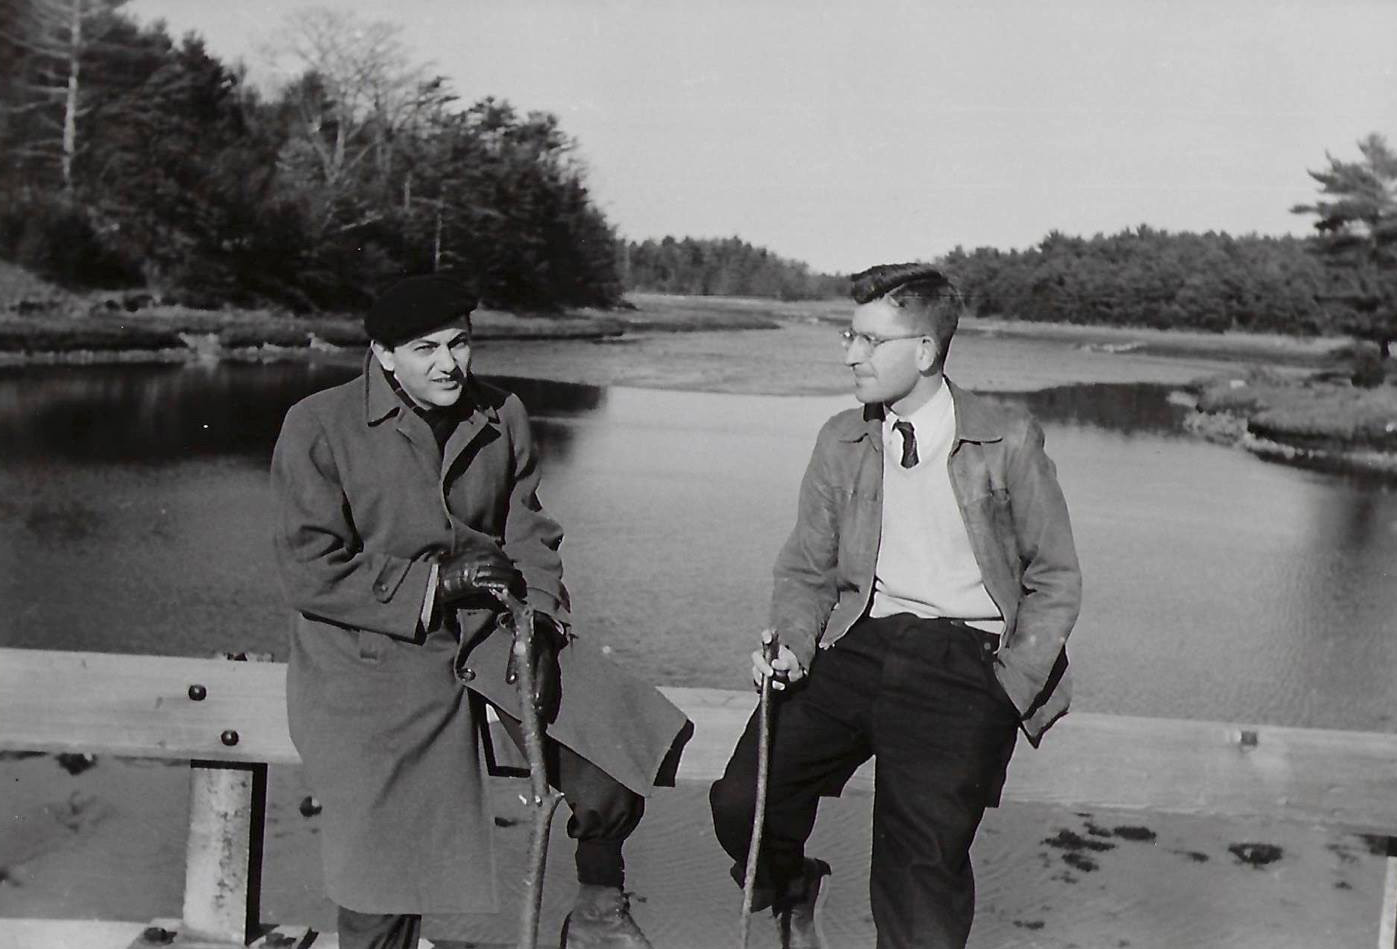
\includegraphics[width=.9\textwidth]{figures/Chomsky_and_Halle_1953_Kittery_Point.jpg}
  \caption{Morris Halle and Noam Chomsky (1953)}
  \label{fig:ch.genphon.kittery}
\end{wrapfigure}
Almost from the beginning, both {\Chomsky} and {\Halle} invoked the names of
figures from the pre-structuralist past as precursors of the sort of
work they were doing. With reference to phonology, {\Sapir} is referred
to in these terms on numerous occasions, as is {\Bloomfield} (in his
practice—e.g., \citealt{bloomfield:menomini_morphophonemics}—though
not with regard to his theoretical
writings). \citet{chomsky63:formalprops} also cites {\Saussure} as
having a picture of linguistic structure somewhat similar to his own,
although {\Chomsky}'s opinion of {\Saussure} has varied significantly over
the years, as described by
\citet[143--155]{joseph02:whitney.to-chomsky} and
\citet{newmeyer13:saussure}. Subsequently, \citet{chomsky66:cartesian}
further emphasized connections between \isi{generative grammar} and the
rationalist philosophy of the Port-Royal grammar, 
Descartes\ia{Descartes, René}, Humboldt\ia{von Humboldt, Wilhelm}, and others.

Claims that this earlier work (whether philosophical or linguistic)
was in some way the source or origin of notions in \isi{generative grammar}
would have to be qualified as mere rationalization \emph{ex post
  facto}. {\Chomsky}'s ideas were developed largely in isolation from the
linguistic tradition. He has emphasized himself \citep[e.g.,
in][]{chomsky79:lg.and.resp} the extent to which his early work was
done completely outside the framework of any particular sort of
linguistics and with little awareness of its specific
antecedents. Similarly, his explorations of early rationalist
philosophy \citep{chomsky66:cartesian} were largely conducted after the essential program of
\isi{generative grammar} was already formulated and well underway.

{\Chomsky}'s discussions of the early rationalists have provoked strong
reactions from historians of science and philosophy, who accuse him of
rewriting the history of ideas as a grand conspiracy to develop the
notion of a \isi{generative grammar}. In fact, however, a more reasonable
assessment is available: the point of his historical interpretations
is that earlier thinkers about language had some very similar insights
to those that motivate work in \isi{generative grammar}, but their point of
view was subsequently replaced by very different ones, and those
insights thus were lost—in the sense that they did not guide
subsequent work.

One attempts to explore the attitudes toward language of earlier
philosophical writers not in order to see them as generative
grammarians \emph{manqués}, or to associate the prestige of their
names with current theory, but because, insofar as their work was
based on similar premises, it may well be of considerable current
relevance. Generative grammar can only stand or fall as a theory of
natural language on the basis of its own explanatory value, but it may
still be quite worthwhile to examine the place of its underlying
assumptions within other, larger philosophical contexts.

The conception of a language as a system of \isi{rules} (rather than a set
of \isi{representations}) which lies at the heart of \posscitet{halle:spr}
\textsl{Sound Pattern of Russian} and his arguments against
structuralist phonemics was naturally quite consistent with {\Chomsky}'s
notions. The \textsl{Morphophonemics of Modern Hebrew} had already
presented a similar picture, and discussions between {\Chomsky} and {\Halle}
during the 1950s had resulted in essential agreement between them
around a program represented by these works and the 1955 model in
\citealt{chomsky85:lslt}. The analysis of \ili{English} proposed by
\citet{chomsky:halle:lukoff} is similarly in line with this conception
of a grammar, though that paper addressed primarily the question of
how to represent \isi{stress}.

\largerpage[-1]
Some aspects of this theoretical program for phonology have clear
antecedents in the work of the Prague school, as is only natural given
{\Halle}'s association with {\Jakobson}. One such part of the theory is the
weight given to the system of \isi{distinctive features} as a theory of
universal phonetics. For various reasons, American structuralists had
never really taken to distinctive feature analyses (with the exception
of a few works such as \citealt{hockett55:manual}, but this
representation was essential to the new theory of generative
phonology. A major point of contention between American structuralist
and early generative theories, in fact, was the insistence of the
former that phonemes should be attended to as unitary elements of
\isi{contrast}, while generative phonology maintained the Jakobsonian view
that the contrastive value of phonemic segments was a byproduct of
contrasts in features. The consequent claim that segments were merely
`unsystematic abbreviations' for complexes of features served as a
major irritant in the new theory for older workers in the field.

\begin{wrapfigure}[13]{r}{.4\textwidth}
  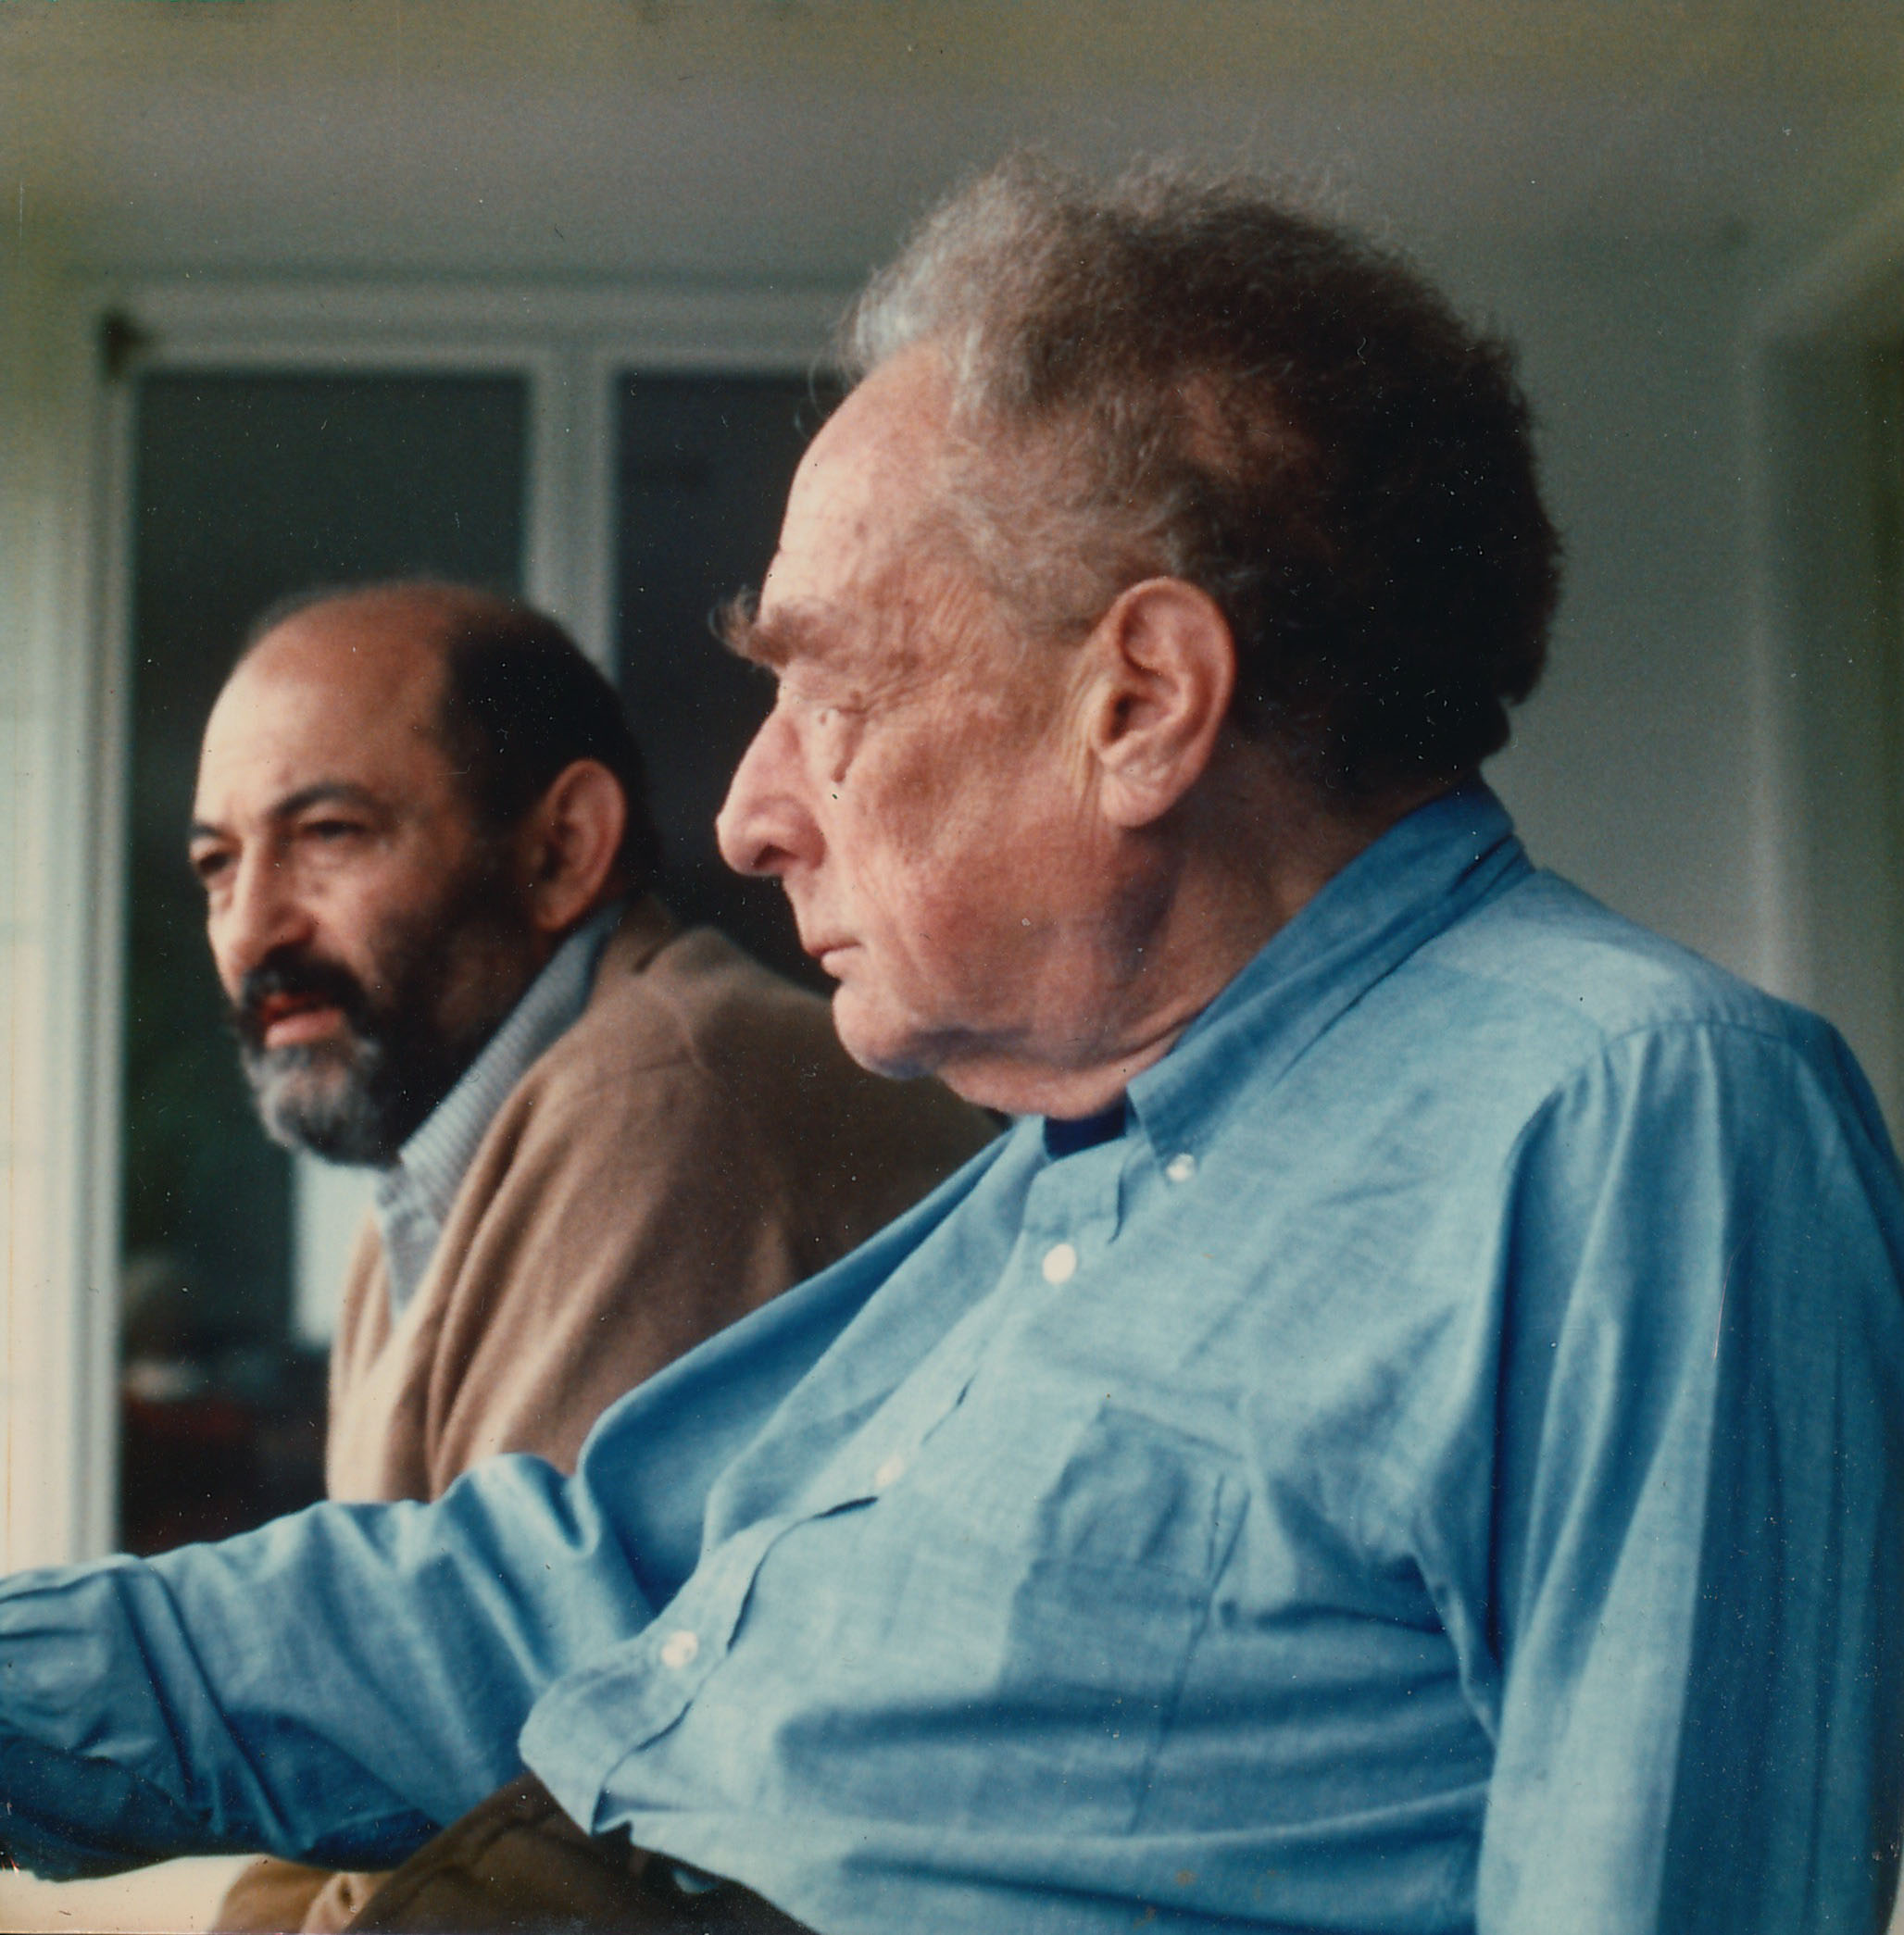
\includegraphics[width=.9\textwidth]{figures/Morris_Roman.jpg}
  \caption{Morris Halle and Roman Jakobson}
  \label{fig:ch.genphon.morris-roman}
\end{wrapfigure}
A primary reason for the attention to features was the prominence
within the theory of the notion of evaluation of grammars. Grammars
were to be formulated in a uniform notation which would make it
possible to compare alternative descriptions of the same facts, and it
was intended that such a comparison would form the basis of a notion
of \isi{explanation} in linguistics. An appropriate \isi{evaluation measure} would
designate one of a class of alternative grammars as preferred over
other available possibilities, and in this way questions concerning
the structural properties of language could be posed in terms of
appropriate characteristics to assign to such a measure. The use of a
feature notation played a central role in early proposals for an
\isi{evaluation measure} over phonological descriptions.

An aspect of language structure which was assumed to be highly valued
was the extent to which \isi{rules} of grammar express `linguistically
significant generalizations' (though it has often been claimed that a
weakness in the theory is the absence of any independent notion of
what these are). Formulating \isi{rules} and \isi{representations} in terms of
features contributes to the assessment of generality,
\citet{halle62:pigg,halle64:bases} argued, because it reflects in the
form of length of statement the generality or \isi{naturalness} of the
classes of segments which an expression refers to: in an adequate
universal feature system, it takes fewer features to characterize more
general natural classes than less general ones. If grammars are
systematically expressed in a notation based on features, they can be
compared in a straightforward way which will reflect the degree of
generalization captured by a given formulation. The role of features
in the theory was thus quite different from that which it served in
Prague school work, but the emphasis on the decomposition of segments
into constituent dimensions of \isi{contrast} is a point of similarity
between the two.

Another Praguian theme in \isi{generative grammar} was a basic concern for
\isi{explanation} in linguistics, and the concomitant search for universal
properties and laws of linguistic structure. As we have seen, both
\isi{universals} and explanatory principles were considered by American
structuralists to be either nonexistent or beyond the scope of
possible research. American linguists sought maximally explicit and
comprehensive descriptions of particular languages, but generally felt
that the only sort of \isi{universals} that could be maintained were
inductive generalizations about the corpus of languages described to
date. This was directly contrary to European practice—which was
generally stigmatized in America as vague and
impressionistic. Generative grammar elevated \isi{explanation} and the
search for \isi{universals} of language to a central place in linguistics,
in the context of a concern for explicitness and formal statement
which could hardly be confused with `mere philosophy'.

In {contrast} with its relation to European linguistics (specifically,
the positions associated with {\Jakobson}) the notion that there is
continuity between early generative phonology and its American
structuralist predecessors is far from obvious, at least to judge by
the rhetoric employed on both sides. There are, nonetheless some
important assumptions of structuralist work which were taken over into
generative phonology with little or no reexamination. One such area is
that of morphological structure.

Structuralism had developed a picture of words as exhaustively
analyzable into sequences of concatenated morphemes: minimal units of
meaningful \isi{sound structure}. Discussion of this conception had
uncovered a large number of important problems: `zero' morphemes,
`portmanteau' morphemes (e.g., \ili{French} \emph{au} for
\emph{à}+\emph{le}), meaningless `morphemes' (such as connectives and
thematic vowels), `morphemes' of replacement (e.g., the plural marker
in \emph{man}/\emph{men}), subtraction, etc. Since no real alternative
existed within \isi{structuralism} to the notion of morphemes as units of
form linked inseparably with units of \isi{meaning}, this picture persisted
even in the face of the unfortunate consequences noted by
\citet{hockett47:survey}, \citet{nida:identification} and others.

The history of this problem is insightfully presented by
\citet{matthews72:infl,matthews93:grammatical_theory}. As he notes,
\isi{generative grammar} simply took over unchanged as part of its notion of
\isi{underlying representation} the conception of morphological structure as
a ``fictitious agglutinating analog'' of the actual forms of a
language \citep[as][put it]{lounsbury53:oneida_verb}. Beginning in the 1960s and
1970s with the work of \citet{matthews65:wp,matthews72:infl}, the
appropriateness of that model of word structure within a generative
grammar has been subject to re-examination on the one hand, and
re-formulation on the other. The bulk of generative descriptions have
been (and continue to be) based on essentially (American)
structuralist assumptions about the morpheme, re-cast for example
within the theory of  Distributed Morphology
\citep{halle.marantz93:bldg20}, although alternatives that replace the
traditional morpheme with an `Inferential/Realizational' framework
\citep{stump01:inflect.morph.book} grounded in {\MatthewsP}' view are also
pursued. These issues fall largely outside the scope of the present
book; see \citealt{sra12:the-morpheme} for some discussion.

As I have argued above, the emphasis of generative phonology broke
with previous work from the beginning by emphasizing the centrality of
\isi{rules} in a theory of language. The focus of early work (which
continues today; though see later in this chapter and
chapter~\ref{ch.otlabphon}) was on the nature and formulation of
\isi{rules}, with questions of representation subordinated to these in the
sense that the \isi{representations} were arranged so as to maximize the
generality of the \isi{rules}. It was taken as at least a goal to reduce any
state of affairs in which two or more phonologically diverse forms
existed for related elements to a description in which a common
underlying form appears, and the \isi{divergence} in surface form is
accounted for by the operation of maximally general \isi{rules}. A rule was
presumed to exist wherever related forms differed in shape, with only
a few irreducible exceptions such as the verb be in \ili{English}—but even
here some made a noble attempt to state apparently suppletive
paradigms as governed by rule \citep[e.g.][]{foley65:sum}. The
underlying forms that were posited were whatever was necessary to
maximize the generality of the \isi{rules} involved.

The emphasis on \isi{rules}, however, is not the only prominent
characteristic of early generative descriptions. Another is the effort
to provide \isi{underlying representation}s from which the last drop of
\isi{redundancy} has been wrung: \isi{representations} which specify the absolute
minimum of information in order to distinguish one morpheme from
another within the system of a given language. In part, this is simply
the continuation of the project which most phonologists since {\Saussure}
have set for themselves. If one conceives of a `phonological'
representation as one which specifies all and only the distinctive or
signalling properties of forms, it follows that all other
(predictable, or redundant) information should be excised from this
representation. More specifically, however, the form in which this
effort was implemented in early generative descriptions derives from
{\Jakobson}'s concerns with \isi{information theory} and the mathematical
theory of communication.

At least in early generative descriptions, this appears particularly
in the way the \isi{phonological system} of a language is presented in the
form of a `\isi{branching diagram}' \citep{dresher.hall21:genphon}. Such a
diagram is an arrangement of the segments of a language into a
sequence of successive choices (each corresponding to a particular
feature), such that at each point the number of elements representing
one possible choice (or feature value) is roughly equal to that
represented by the opposite choice. The overall set of distinctions
among segments is thus organized so as to minimize not simply
predictable specifications, but more particularly the number of actual
specifications necessary to identify uniquely any given (underlying)
segment.

Superficially, at least, the motivation for branching diagrams of
phonological segment inventories seemed to follow from the more
general task of evaluation of grammars: if the evaluation metric for
grammars is to be based on the measure of length of expression when
descriptions are formulated in a standard notation, and if feature
notation is an appropriate way to represent segments and classes of
segments, then it follows that a grammar should be organized so as to
minimize the number of features necessary to characterize any
individual segment.

There is an important flaw in this argument, however. The claim of
shortness of expression as an appropriate evaluation procedure is not
really an empirical proposal about the nature of language; it is,
rather, a framework within which such proposals can be made. Any
expression can trivially be made to be shorter than any other by the
choice of an appropriate set of abbreviatory conventions: proposals
that one formally characterized type of rule rather than another is
more natural in human languages are then made in the form of proposals
for the set of such abbreviatory conventions. Much of generative
phonology up through the appearance of \citealt{spe} and work
immediately deriving therefrom was explicitly devoted to just this
task. The assumption that, given a set of \isi{notational conventions} for
\isi{rules}, length as a function of the number of specified features can be
taken as an appropriate measure of generality for \isi{rules}, however, does
not at all entail the conclusion that the number of feature
specifications in the lexicon should be similarly minimized. In fact,
there is little if any connection between the notion that \isi{rules} should
be formulated in maximally general terms and a requirement that the
lexicon should be specified with as few features as possible.

Especially during the 1960s, generative grammars were concerned with
various aspects of the problem of eliminating as many features as
possible from \isi{underlying representation}s. This was done by optimizing
the distribution of contrasts, in association with a set of morpheme
structure \isi{rules} which filled in the redundant features. In part, this
project of extracting as much \isi{redundancy} as possible followed from the
considerations of evaluation discussed above, but it was also simply
assumed (as part of generative phonology's Jakobsonian heritage) that
this was part of what one did when one described the phonology of a
language. The requirement of redundancy-free underlying
\isi{representations}, however, and the status of \isi{morpheme structure rules}
(\emph{vis-à-vis} ordinary \isi{phonological rules}) raised a number of
strictly mechanical problems (some of which were reviewed by
\citet{stanley67:redundancy}). These problems are not reviewed in
detail here, since their relevance was confined to a fairly narrow
time period.

In is interesting to note that a concern for \isi{morpheme structure rules}
and the elimination of \isi{redundancy} gradually disappeared from
generative descriptions, without ever being effectively renounced as a
theoretical concern. The presentation of `branching diagrams' for the
segments of a language is a practice which fell out of use by the
mid-1960s, and concern for the statement of \isi{redundancy rules} more or
less disappears by the end of the decade. It might be possible to
attribute this change to proposals such as those of
\citet{stanley67:redundancy} and the last chapter of \citet{spe}, both
of which argued (for somewhat different reasons) that lexical
\isi{representations} should after all be fully specified, and that
\isi{redundancy} should be treated in other ways. This does not seem to be
the entire story, however.

Early concern for evaluation procedures, in the form of specific
arguments that (in an appropriate notation) shorter descriptions could
be empirically validated as correct, turned out to be something of a
dead end. Virtually the only actual argument of this form in the
literature is {\Chomsky} and {\Halle}'s often repeated citation of the
differences among \emph{brick} (an occurring word in \ili{English}),
\emph{bnick} (an impossible word in \ili{English}) and \emph{blick} (a
possible, but non-occurring word in \ili{English}; it is amusing to note
that, apparently unknown to {\Chomsky} and {\Halle}, \emph{blik} had been
employed in 1950 in ``Theology and Falsification'' as a nonce word by
the philosopher \name{R. M.}{Hare} in a debate with \name{Antony}{Flew}, designating a
worldview which is meaningful but unverifiable and unfalsifiable). In
the absence of further convincing examples \citep[but see][ch. 6 for
an attempt to construct another]{sra74:orgphon} , the appeal of
feature counting went away and, with it, much of the apparatus that
was intended to support it—not with a bang, but a whimper.

The theoretical problems of the `classical' period of generative
phonology (up to the early 1970s), then, were fundamentally problems
of the nature of \isi{rules}: the design of an appropriate notation for
expressing \isi{rules}, the choice of an adequate set of abbreviatory
conventions for sets of \isi{rules}, the formulation of principles governing
the ordering and other interactions of \isi{rules} within a grammar. Even
the central representational issue of the period, the elimination of
\isi{redundancy} from underlying forms, was typically posed as a matter of
the status and formulation of \isi{morpheme structure rules} or some
replacement for these. In this context, phonological (and even
phonetic) \isi{representations} were simply assumed to have the properties
necessary to enable the \isi{rules} to function in a maximally general way.

Not long after the appearance of \textsl{The Sound Pattern of English}
in 1968, however, a number of phonologists began to raise objections
from several sides to then-current practice. Most of these objections
had their origins in a renewed inquiry into the properties of
\isi{representations} per se, and it is to these developments that we turn
in the following chapters.

%%% Local Variables: 
%%% mode: latex
%%% TeX-master: "/Users/sra/Dropbox/Docs/Books/P20C_2/LSP/main.tex"
%%% End: 
